%
% For tracking purposes - this is V2.0 - May 2012

\documentclass{ieeeconf}
\usepackage[colorinlistoftodos,obeyFinal]{todonotes}                            
%\usepackage{caption}
\usepackage{fainekos-macros}
\usepackage[]{algorithm2e}
\usepackage{amsmath} % assumes amsmath package installed
\usepackage{amssymb}  % assumes amsmath package installed
\usepackage{graphicx}
\usepackage{tikz}
\usetikzlibrary{arrows}
\usepackage{ifthen}
\usepackage{mathtools}
\usepackage{stmaryrd}
\usepackage{csquotes}
\usepackage{xargs}                      % Use more than one optional 
\usepackage{subcaption}
\usepackage{textcomp}
%\usepackage[pdftex,dvipsnames]{xcolor}  % Coloured text etc. 

\newcommand{\rob}{\rho}
\newcommand{\robf}{\rho_{\formula}}
\newcommand{\robfa}{\rho_{\formula_1}}
\newcommand{\robfb}{\rho_{\formula_2}}
\newcommand{\srob}{\tilde{\rob}}
\newcommand{\srobf}{\srob_\formula}
\newcommand{\smax}{\widetilde{\max}}
\newcommand{\smin}{\widetilde{\min}}
\newcommand{\sdist}{\widetilde{\mathbf{dist}}}

\newcommand{\sd}{\rho}
\newcommand{\bs}[2]{\ll\!#1,#2\!\gg}
\newcommand{\rd}[2]{\ll\!#1,#2\!\gg_\Re}
\newcommand{\rs}[2]{\ensuremath{\llbracket #1,#2 \rrbracket}}
\newcommand{\cl}[1]{\overline{#1}}
\newcommand{\Ltf}{\Lc_t(\formula)}
\newcommand{\Ltnp}{\Lc_t(\lnot p)}
\newcommand{\Ltp}{\Lc_t(p)}
\newcommand{\Lrf}{\Lc_{\Re_\Fc}}

%for blank footnote
\usepackage{lipsum}
\newcommand\blfootnote[1]{%
  \begingroup
  \renewcommand\thefootnote{}\footnote{#1}%
  \addtocounter{footnote}{-1}%
  \endgroup
}

% remove acm copyright
\usepackage{etoolbox}
\makeatletter
\patchcmd{\maketitle}{\@copyrightspace}{}{}{}
\makeatother

\usepackage{xcolor}
\newcommand\ypcomment[1]{\textcolor{blue}{\textbf{#1}}}
\usepackage{url}
%\usepackage{hyperref}
% Control spacing...
%\setlength{\marginparwidth}{4cm}
%\setlength{\textfloatsep}{2pt}
\linespread{0.97}
%\thickmuskip=0mu
%\usepackage[margin=0.7in]{geometry}
\begin{document}

%\CopyrightYear{2017} \setcopyright{acmcopyright}
%\conferenceinfo{ICCPS '17,}{April 18--21, 2017, Pittsburgh, Pennsylvania, USA.}
%\isbn{978-1-4503-3955-1/16/04}\acmPrice{\$15.00}
%\doi{http://dx.doi.org/10.1145/2883817.2883841}

%Authors, replace the red X's with your assigned DOI string.

\title{Goal Revision: Robust Control of Systems with Temporal Logic Specifications}

%\author{
	% 1st. author
%	\alignauthor
%	Yash Vardhan Pant\thanks{The authors contributed equally.}, Houssam Abbas\footnotemark[1], Rahul Mangharam\\
%	\affaddr{Department of Electrical and Systems Engineering}\\
%	\affaddr{University of Pennsylvania, Philadelphia, PA, USA}\\
%	\email{\{yashpant, habbas, rahulm\}@seas.upenn.edu}%
%}

\author{Houssam Abbas$^{*}$, Yash Vardhan Pant$^{*}$, Rahul Mangharam% <-this % stops a space
\thanks{*The authors contributed equally.}% <-this % stops a space
\thanks{Department of Electrical and Systems Engineering, University of Pennsylvania, Philadelphia, PA, USA.}%
\thanks{{\tt\small $\{$habbas, yashpant, rahulm$\}$@seas.upenn.edu}}%
}




%\author{
%\alignauthor
%	\affaddr{University of Pennsylvania, Philadelphia, PA, USA}\\
%	\email{\{piggies1,2,3\}@seas.upenn.edu}%
%Yash Vardhan Pant\thanks{The authors contributed equally.}\and Houssam Abbas\footnotemark[1] \and Rahul Mangharam \\ % \\
%\affaddr{Department of Electrical and Systems Engineering}\\
%	\affaddr{University of Pennsylvania, Philadelphia, PA, USA}\\
%	\email{\{piggies1,2,3\}@seas.upenn.edu}% 
%\thanks{This work was supported by STARnet a Semiconductor Research
%Corporation program sponsored by MARCO and DARPA, NSF MRI-0923518 and the US Department of Transportation University Transportation Center Program}% <-this % stops a space
%\thanks{The Department of Electrical and Systems Engineering, University of Pennsylvania, Philadelphia, U.S.A.
%        {\small
%        \{yashpant,habbas,rahulm\}@seas.upenn.edu}}%
%}


\maketitle
\blfootnote{This work was supported by STARnet a Semiconductor Research
Corporation program sponsored by MARCO and DARPA, NSF MRI-0923518 and the US Department of Transportation University Transportation Center Program.}

%\color{blue}{Shizzle}


\input{Abstract}
\input{Morari}
\section{Robustness of MTL formulae}
\label{sec:robust semantics}

Consider a discrete-time dynamical system $\Sys$ given by 
\begin{equation}
\label{eq:xt}
x_{t+1} = f(x_t,u_t)
\end{equation}
where $x \in X \subset \Re^n$ is the state of the system and $u \in U \subset \Re^m$ is its control input.
The system's initial state $x_0$ takes value from some initial set $X_0 \subset \Re^n$.
Given an initial state $x_0$ and a control input sequence $\inpSig = (u_0,u_1,\ldots), u_t \in U$, a trajectory of the system is the unique sequence of states $\sstraj = (x_0,x_1,\ldots)$ s.t. for all $t$, $x_t$ is in $X$ and it obeys \eqref{eq:xt} at every time step.
We will use $\TDom$ to abbreviate the time domain $\{0,1,2,\ldots\}$.
All temporal intervals that appear in this paper are discrete-time, e.g. $[a,b]$ means $[a,b] \cap \TDom$. 
For an interval $I$, we write $t+I = \{t+a \such a \in I\}$.
The set of subsets of a set $S$ is denoted $\Pc(S)$.
The signal space $\SigSpace$ is the set of all signals $\sstraj: \TDom \rightarrow X$.
The max operator is written $\sqcup$ and min is written $\sqcap$.

\subsection{Metric Temporal Logic}
\label{sec:mtl}
The controller of $\Sys$ is designed to make the closed loop system \eqref{eq:xt} satisfy a specification expressed in Metric Temporal Logic (MTL)~\cite{Ouaknine08_RecentResultsMTL}.
MTL allows one to formally express complex reactive specifications, beyond stability, trajectory tracking and the like.
%See examples \eqref{eq:rule1mtl} and \eqref{eq:rule3mtl}.

Formally, let $AP$ be a set of atomic propositions, which can be thought of as point-wise constraints on the state of the system.
An MTL formula $\formula$ is built recursively from the atomic propositions using the following grammar:
\[\formula \defeq \top|p|\neg \formula | \formula_1 \lor \formula_2 | \formula_1 \land \formula_2 | \formula_1 \until_I \formula_2\]
where $I \subset \Re$ is a time interval.
Here, $\top$ is the Boolean True, $p$ is an atomic proposition, $\neg$ is Boolean negation, $\lor$ and $\land$ are the Boolean OR and AND operators, respectively, and $\until$ is the Until temporal operator.
Informally, $\formula_1 \until_I \formula_2$ means that $\formula_1$ must hold \textit{until} $\formula_2$ holds, and that the hand-over from $\formula_1$  to $\formula_2$ must happen sometime during the interval $I$.
The implication ($\implies$), Always ($\always$) and Eventually ($\eventually$) operators can be derived using the above operators.

Formally, the \textit{pointwise semantics} of an MTL formula define what it means for a system trajectory $\sstraj$ to satisfy the formula $\formula$.
Let $\Oc: AP \rightarrow \Pc(X)$ be an \textit{observation} map for the atomic propositions.
The boolean truth value of a formula $\formula$ w.r.t. the trajectory $\sstraj$ at time $t$ is defined recursively.
\begin{definition}[MTL semantics]
	\label{def:boolean sat}
	\begin{eqnarray*}
		\label{eq:boolean sat}
		(\sstraj,t) \models \top &\Leftrightarrow& \top
		\\
		\forall p \in AP, (\sstraj, t) \; \models_\Oc p &\Leftrightarrow& x_t \in \Oc(p)
		\\
		(\sstraj,t) \models_\Oc \neg \formula&\Leftrightarrow& \neg (\sstraj,t) \models_\Oc \formula
		\\
		(\sstraj,t) \models_\Oc \formula_1 \lor \formula_2 &\Leftrightarrow& (\sstraj,t) \models_\Oc \formula_1 \lor (\sstraj,t) \models_\Oc \formula_2
		\\
		(\sstraj,t) \models_\Oc  \formula_1 \land \formula_2&\Leftrightarrow& (\sstraj,t) \models_\Oc \formula_1 \land (\sstraj,t) \models_\Oc \formula_2
		\\
		(\sstraj,t) \models_\Oc \formula_1 \until_I \formula_2 &\Leftrightarrow& \exists t' \in t+I .  (\sstraj,t') \models_\Oc \formula_2  
		\\
		&& \, \land \forall t'' \in (t,t'), \;\; (\sstraj,t'') \models_\Oc \formula_1 
	\end{eqnarray*}
\end{definition}
As $\Oc$ is fixed in this paper, we drop it from the notation.
We say $\sstraj$ satisfies $\formula$ if $(\sstraj,0) \models \formula$.
All formulas that appear in this paper have bounded temporal intervals: $ 0\leq \inf I < \sup I < +\infty$.
To evaluate whether such a formula $\formula$ holds on a given trajectory, only a finite-length prefix of that trajectory is needed.
Its length can be upper-bounded by the \textit{horizon} of $\formula$, $hrz(\formula)$, calculable as shown in~\cite{Dokhanchi14_OnlineMonitoring}. 
For example, the horizon of $\eventually_{[2,4]}p$ is 6.

\subsection{Robust semantics of MTL}
\label{sec:rob sem}
Designing a controller that satisfies the MTL formula $\formula$\footnote{Strictly speaking, a controller such that the closed-loop satisfies the formula.} is not always enough.
In a dynamic environment, where the system must react to new unforeseen events, it is useful to have a margin of maneuverability.
That is, it is useful to control the system such that we \textit{maximize} our degree of satisfaction of the formula.
When unforeseen events occur, the system can react to them without violating the formula.
This degree of satisfaction can be formally defined and computed using the robust semantics of MTL.
Given a point $x \in X$ and a set $A \subset X$, $\dist(x,A) \defeq \inf_{a \in \cl{A}}|x-a|_2$ is the distance from $x$  to the closure $\cl{A}$ of $A$.
\begin{definition}[Robustness\cite{FainekosP09tcs}]
	\label{def:robustness estimate}
	The \emph{robustness} of $\varphi$ relative to $\sstraj$ at time $t$ is recursively defined as 
	\begin{eqnarray*}
		\label{eq:robustness estimate}
		\rob_{\top} (\sstraj,t) &=& +\infty
		\\
		\forall p \in AP, \;  \rob_{p} (\sstraj,t) &=& \left \lbrace \begin{matrix}
			\dist(\stPt_t, \stSet \setminus \Oc(p)), &\text{if } \stPt_t \in \Oc(p)
			\\
			-\dist(x_t, \Oc(p)), &\text{if } \stPt_t \notin \Oc(p)						
		\end{matrix} \right.
		\\
		\rob_{\lnot \formula} (\sstraj,t) &=& - \rob_{\formula} (\sstraj,t)
		\\
		\rob_{ \formula_1 \lor \formula_2} (\sstraj,t) &=& \rob_{\formula_1} (\sstraj,t) \sqcup \rob_{\formula_2} (\sstraj,t) 
		\\
		\rob_{ \formula_1 \land \formula_2} (\sstraj,t) &=& \rob_{\formula_1} (\sstraj,t) \sqcap \rob_{\formula_2} (\sstraj,t) 
		\\
		\rob_{ \formula_1 \until_I \formula_2} (\sstraj,t) &=& \sqcup_{t' \in t+_{\TDom}I} \left(\rob_{\formula_2} (\sstraj,t') \bigsqcap \right.
		\\
		&& \left. \sqcap_{t'' \in [t,t')}   \rob_{\formula_1} (\sstraj,t'') \right) 
	\end{eqnarray*}
	When $t=0$, we write $\robf(\sstraj)$ instead of $\robf(\sstraj,0)$.
\end{definition}

\section{The Goal Revision framework}

For autonomous systems with higher level specifications, situations may arise when satisfying all of the high level specifications is not possible. An example would be,
...
In such scenarios, it is preferable to satisfy the more important specifications while possibly violating ones with lesser importance. The automata of Fig.\ref{} (\ypcomment{The automata you drew to show me the preference order of specs})  shows the preference of satisfaction of subformulae that make up the overall specification of the form:
\begin{equation}
\formula = \always (\Phi_1 \land \Phi_2 \land \Phi_3)
\end{equation}







With specifications written in MTL, a bottom-up view of the goal revision problem leads us to three important sub-problems that need to be solved:

\begin{itemize}
\item \textit{Control for satisfaction of one MTL specification}: Before we can move on to the complete goal revision problem, the question arises on how can we control a system to satisfy a given MTL specification. Existing approaches involve MILP formulations of MTL specifications \cite{Raman14_MPCSTL}, but do not scale well as formulae become complex. On going work on maximizing a smooth approximation of MTL robustness \cite{PantAM17_SmoothOpTechRpt} has led to promising results with regards to overall performance, run-times and scalability of the method beyond MILP based approaches. The method applies to time bounded MTL formulae and like existing approaches, requires solving for a control horizon that is as long as the formula length itself, which is not ideal for real-time implementations. There is also a need to extend the methods to incorporate uncertainties in the knowledge of the state of the system and the environment.

\item \textit{Receding Horizon control for a given MTL specification}: For a more tractable control algorithm, it is important to be able to solve a control problem with a look-ahead horizon smaller than the MTL formula's time horizon. No current approach does this while guaranteeing the important \textit{recursive feasibility} like property which is common in MPC. On going work focuses on using the concept to \textit{feasibility envelopes}\cite{Belta_FE_CDC16} for MTL formulae to enforce a \textit{terminal} constraint on the receding-horizon control problem to guarantee weaker form of recursive feasibility. 

\item \textit{The goal revision problem}: \ypcomment{Habbas lay this down?}

\end{itemize}

\subsection{Robustness maximization for Control of systems with MTL specifications}
\newcommand{\fe}{f_\varepsilon}

For the robust semantics of MTL formula as defined in Sec.\ref{sec:robust semantics}, we come up with a smooth ($\mathbf{C}^{\infty}$) approximation of the robustness $\rob_\formula$, $\srob_\formula$ (details can be found in \cite{PantAM17_SmoothOpTechRpt}). This approximation is then maximized to compute the control sequence for a given system to satisfy the time-bounded MTL specification $\formula$ (with horizon $N$ time-steps). The optimization problem is:
\begin{subequations}
	\label{eq:general_ctrl}
	\begin{align}
	P_{\srob}:\, \max_{\mathbf{u}}\, & \srob_{\formula}(\sstraj) - \gamma \sum_{k=0}^{N-1} l(x_{k+1},u_{k}) \label{eq:general ctrl obj}\\
	\text{s.t. } & x_{k+1} = f(x_k,u_k), \, \forall k=0,\dotsc,N-1 \label{eq:general ctrl dyn}\\
	& x_k \in X, \, \forall k=0,\dotsc,N \label{eq:general ctrl X}\\
	& u_k \in U, \, \forall k=0,\dotsc,N-1 \label{eq:general ctrl U}\\
	& \delta \srob_{\formula}(\sstraj) \geq \delta \epsilon_{\text{min}} \label{eq:general ctrl pos rob}
	\end{align}
\end{subequations}

%We want to use established, powerful gradient descent algorithms \cite{Polak97_Optim}, rather than heuristics like Simulated Annealing \cite{kirkpatrickV_SA83}. 
Here, $\mathbf{u} = (u_0,\ldots,u_{N-1})$, 
$l(x_{k+1},u_{k})$ is a control cost, e.g. the LQR cost $x_k'Qx_k + u_k'Ru_k$,
and $\gamma \geq 0$ is a trade-off weight. 
The scalar $\epsilon_{\text{min}} \geq 0$ is a desired minimum robustness. 
If $\delta = 0$, then this constraint is effectively removed, while $\delta=1$ enforces the constraint.


For an online implementation of the controller, this one-shot optimization problem can be solved repeatedly at each time step while adding equality constraints to fix the variables to their values in the past time steps. A couple of examples show the performance of this approach:

%\subsubsection{Simulation Results}
\begin{exmp}
\label{ex:toyproblem}
The planar linear system $x_{k+1} = x_k + u_k$ is controlled
%\begin{equation}
%\label{eq:PointMass}
%x_{k+1} = x_k + u_k
%\end{equation}
to satisfy the specification
\[\formula = \always_{[0,20]} \neg (x \in \text{Unsafe}) \land \eventually_{[0,20]} (x \in \text{Terminal})\]
%with the sets $\text{Unsafe}=[-1,1]^2$ and $\text{Terminal}=[2,2.5]^2$. 
%The state space is $X=[-2.5,2.5]^2$, $U=[-0.5,0.5]^2$.
%Unless otherwise indicated, $\gamma=\delta=0$ in Eq. \eqref{eq:general_ctrl} to focus on robustness maximization in this illustrative example. 
%Experiments were run on a quad-core Intel i5 3.2GHz processor with 24GB RAM, running MATLAB 2016b. 
Comparisons are done with the tool BluSTL, which implements the MILP approach of ~\cite{Raman14_MPCSTL} and is used in the experiments.
It has two modes of operation: mode (B) or \textit{Boolean}, which aims at satisfying the specification without maximizing its robustness, and mode (R) or \textit{Robust}, which attempts to maximize robustness. 
The proposed SOP method optimizes robustness and so naturally runs in mode (R).
SOP emulates mode (B) by terminating the optimization as soon as $\srobf \geq \epsilon_{\text{Meyer}}$, which implies $\rob_{\formula} \geq 0$. $\epsilon_{\text{Meyer}}$ can be computed explicitly using the approach in the online report \cite{PantAM17_SmoothOpTechRpt}.

%The goal of $P_{\srob}$ with $\gamma=0$ is to find a trajectory that maximizes $\srob$, hence there is no need for the additional lower bound constraint (Eq. \ref{eq:general ctrl pos rob}) on $\srob$. This is why we also set $\delta=0$ in $P_{\srob}$ for all examples that follow.

\textbf{Results}.
Fig. \ref{fig:toy control} shows the trajectories of length $N=20$ obtained by SOP and BluSTL in modes (B) and (R), starting from the same initial point $x_0=[-2,-2]'$.
Both BluSTL(B) and SOP(B) produce satisfying trajectories. 
The trajectory from SOP(R) ends in the middle of the terminal set, resulting in a higher robustness than mode (B), as expected. 
In mode (R), BluSTL could not finish a single instance of robustness maximization within 100 hours on both the above machine and on a more powerful 8 core Intel Xeon machine with 60GB RAM, leading us to believe that the corresponding MILP was not tractable.
 
SOP(R, $\gamma\!=\!0.1$) takes into account a control cost $l(x_k,u_k) = ||x_k||_{2}^2$ that penalizes longer trajectories.
The resulting trajectory is shorter but has a lower robustness than SOP(R, $\gamma = 0$), ($0.236$ vs $0.247$).

%For further evaluation, we ran 100 instances of the problem, varying the trajectory's initial state in $[-2.5,-1.5] \times [-2.5,2.5]$. 
%We also varied the formula horizon $N$ (and hence the size of the problem) from $20$ to $200$ time steps. 
Table \ref{tbl:time_performance_toy} shows the execution times. 


\textbf{Analysis.}
As seen in Table \ref{tbl:time_performance_toy}, SOP is consistently faster than BluSTL in Boolean mode, and displays smaller variances in runtimes. 
Note also that the problem solved here is very similar to the one used in \cite{Saha_acc16}, which uses another MILP-based method. 
While the underlying dynamics differ and their numbers are reported on a more power machine, 
SOP numbers compare favourably with those in \cite{Saha_acc16}.

In (R) mode, across 100 experiments, SOP has an average $\rob_{\formula}=0.247$ with a standard deviation less than $0.005$. 
This gets very close to the upper bound on robustness, which is 0.25.
This bound is achieved by a trajectory reaching (in $<20$ time steps) the center of the Terminal set while remaining more than 0.25 distant from Unsafe. 
%Also with this additional knowledge of the global optima upper bound, the SOP method in \textit{robust} mode can be made a lot faster by specifying an exit condition based on a upper threshold of $\srob_{\formula}$ attained at any iteration of the SOP method. While for brevity we do not include results with this additional stopping criteria, it was observed that for an upper bound value of $\srob_{\formula}=0.24$, an average speed up of about $4$-times was observed for $N=20$ and $2$-times for $N=200$ while resulting an average robustness value achieved of $\rob_{\formula} = 0.235$. This shows that with the iterative nature of SQP, we can trade-off performance for improved execution times.
\end{exmp}

\begin{figure}[t]
\centering
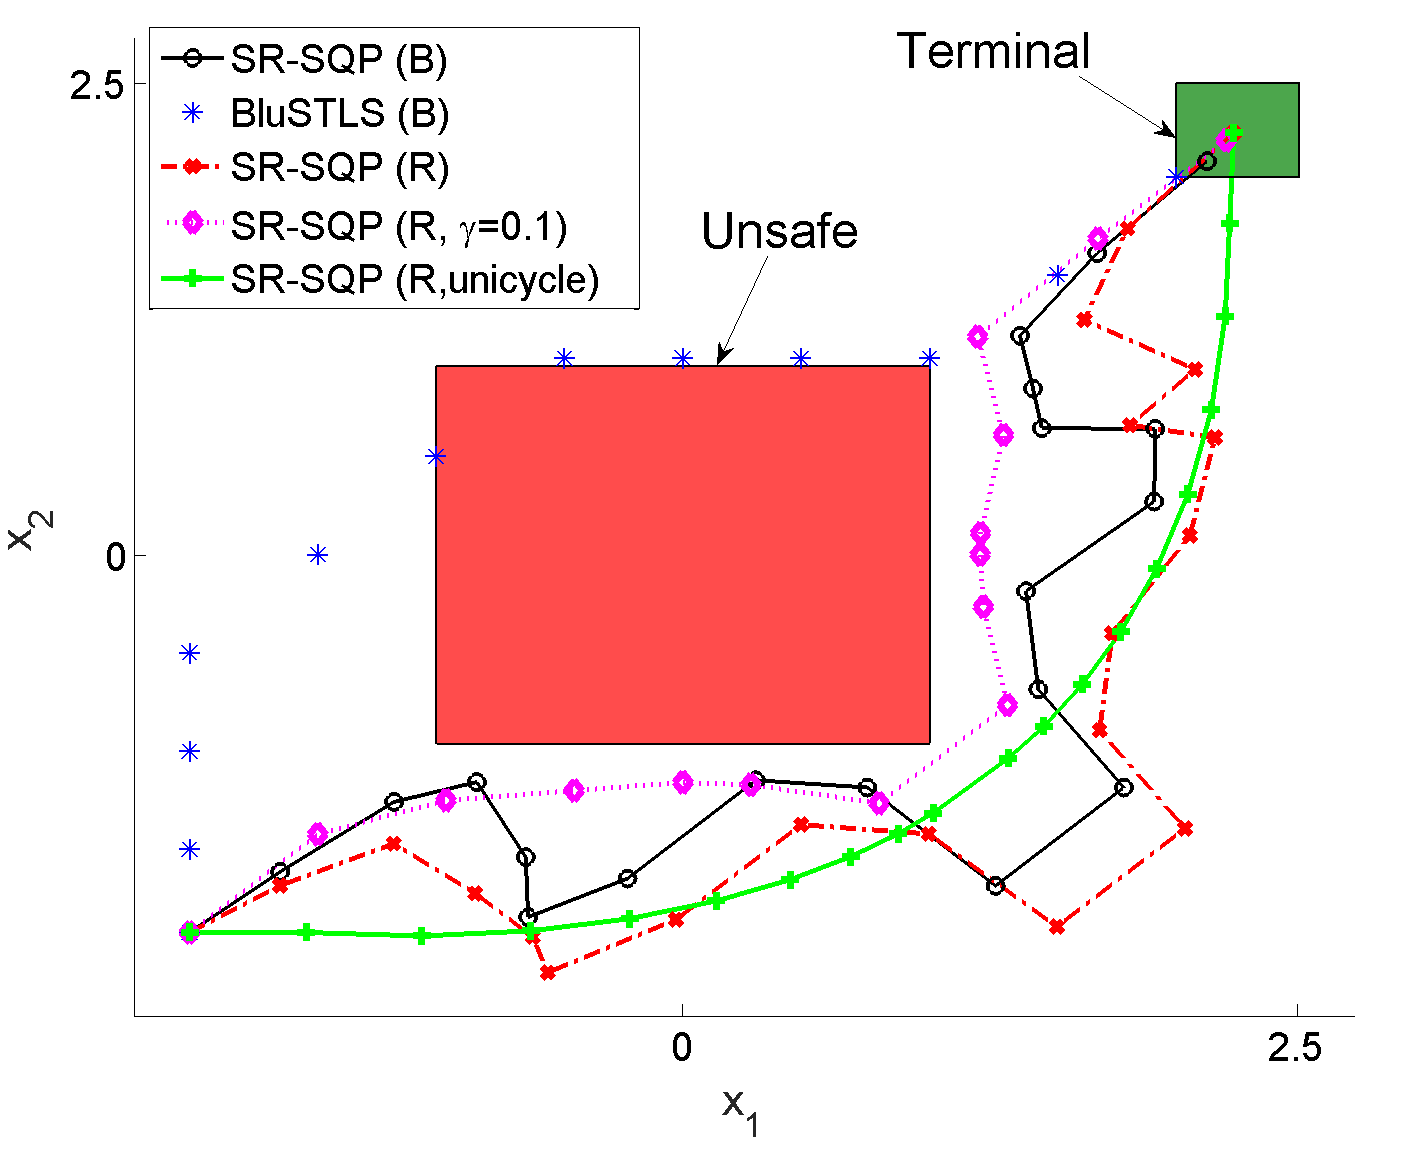
\includegraphics[width=0.49\textwidth]{figures/ToyExUni_alternate_scissored.pdf}
\vspace{-20pt}
\caption{{\small The first 4 trajectories are for Example \ref{ex:toyproblem}. The last trajectory is for the system with the non-linear unicycle dynamics. Colors in online version.}}
\label{fig:toy control}
\vspace{-10pt}
\end{figure}


\begin{table}[tb]
\small
\begin{center}
\caption{{\small Example \ref{ex:toyproblem}. Runtimes (mean and standard deviation, in seconds) for Smooth Operator (SOP) and BluSTL (BlS) in modes (B) and (R), over 100 runs with random initial states and different formula horizons $N$. BluSTL(R) did not finish (see text).}}
\vspace{-5pt}
\label{tbl:time_performance_toy}
\begin{tabular} {|c|c|c|c|c|}
	\hline
	N & BlS(B) & SOP(B) & BlS(R) & SOP(R) \\ \hline
	20 & $0.96 \pm 0.82$ &  $\mathbf{0.31 \pm 0.13}$  & NA & $3.30 \pm 1.25$ \\ \hline
	30 & $1.37 \pm 1.72$ &  $\mathbf{0.33 \pm 0.25}$  & NA & $5.85 \pm 2.74$\\ \hline
	40 & $3.86 \pm 5.10$ &  $\mathbf{0.60 \pm 0.29}$  & NA & $12.36 \pm 6.04$\\ \hline
	50 & $4.36 \pm 12.97$&  $\mathbf{0.74 \pm 0.30}$ & NA & $30.05 \pm 18.23$\\ \hline
	100& $16.77 \pm 27.84$ & $\mathbf{1.21 \pm 0.25}$ & NA & $69.70 \pm 13.16$ \\ \hline
	200& $53.88 \pm 14.18$& $\mathbf{4.19 \pm 1.18}$ & NA & $126.11 \pm 20.43$ \\ \hline
\end{tabular}	
\end{center}
\end{table}

\begin{exmp}
We also tested this approach on an example for 2 quad-rotors with a given complex specification. Playback of the resulting trajectories can be seen in \protect\url{https://youtu.be/FU3Rg1Jb7Fw}. More details in \cite{PantAM17_SmoothOpTechRpt}.
\end{exmp}

\subsection{Ongoing work}
\begin{itemize}
\item Feasibility envelopes and robustness maximization for receding horizon control with MTL specifications.
\item Goal revision.
\item Scalable and fast GPU implementation.
\end{itemize}
%\cite{Abbas14_MTLDescent}

%\addtolength{\textheight}{-12cm}   % This command serves to balance the column lengths
% on the last page of the document manually. It shortens
% the textheight of the last page by a suitable amount.
% This command does not take effect until the next page
% so it should come on the page before the last. Make
% sure that you do not shorten the textheight too much.
\bibliographystyle{IEEEtran}
\bibliography{iccps2017,hscc17,hscc2016,fainekos_bibrefs}
\end{document}